\documentclass{ximera}

\usepackage{microtype}
\usepackage{tikz}
\usepackage{tkz-euclide}
\usetkzobj{all}
\tikzstyle geometryDiagrams=[ultra thick,color=blue!50!black]

\renewcommand{\epsilon}{\varepsilon}



\title{Lines, angles, and areas in central projection}

\begin{document}
\begin{abstract}
  Here we look at lines, angles, and areas in central projection coordinates. 
\end{abstract}
\maketitle

\section{Central projection preserves lines}

We all probably realize that you can't make a perfect flat map of our
spherical world.

What this means is that either great circular arcs on the sphere won't
correspond to straight lines on the map, or angles on the sphere be
equal to the corresponding angles on the map.

We do the next best thing---we make two maps of the sphere!  One map
has the property that straight lines on the map correspond to shortest
paths, and the other map has the property that angles are faithfully
represented. We will now show that in central projection, straight
lines correspond to shortest paths, but angles are not faithfully
represented.






\begin{problem}
  Show that ``lines'' in $K$-geometry correspond to actual lines in
  $(x_{c},y_{c})$-coordinates under central projection.

\begin{hint}
  To intersect two surfaces, say $f(x,y,z)=a$ and $g(x,y,z)=b$,
  simply examine
  \[
  f(x,y,z)-g(x,y,z) = a-b.
  \]
\end{hint}

\begin{hint}
  Explain why intersecting the $K$-surface
  \[
  1 = K\left(x^2+y^2\right) + z^2 
  \]
  with the plane
  \[
  ax+by+cz = 0
  \]
  produces a $K$ geometry line.
\end{hint}

\begin{hint}
  Use the projection formulas
  \begin{align*}
      x &= \frac{x_c}{\sqrt{K\left(x_c^2 + y_c^2\right)+1}},\\
      y &= \frac{y_c}{\sqrt{K\left(x_c^2 + y_c^2\right)+1}},\\
      z &= \frac{1}{\sqrt{K\left(x_c^2 + y_c^2\right)+1}},
  \end{align*}
  and note that these points are \textit{necessarily} on the surface
  \[
  1 = K\left(x^2+y^2\right) + z^2.
  \]
\end{hint}

\begin{freeResponse}
  Let's start by intersecting the surfaces
  \[
  K\left(x^2+y^2\right)+z^2=1\qquad\text{and}\qquad ax+by+cz=0,
  \]
  where the latter is a plane passing through the origin. Write
  \[
  K\left(x^2+y^2\right) + z^2- ax- by-cz=1.
  \]
  Now use the projection formulas. Since these formula necessarily
  produce points on the surface
  \[
  1 = K\left(x^2+y^2\right) + z^2,
  \]
  we may replace $K\left(x^2+y^2\right) + z^2$ with $1$ and write
  \begin{align*}
    1-\frac{ax_c}{\sqrt{K\left(x_c^2 + y_c^2\right)+1}}- \frac{by_c}{\sqrt{K\left(x_c^2 + y_c^2\right)+1}}-\frac{c}{\sqrt{K\left(x_c^2 + y_c^2\right)+1}} &=1\\
    -\frac{ax_c}{\sqrt{K\left(x_c^2 + y_c^2\right)+1}}- \frac{by_c}{\sqrt{K\left(x_c^2 + y_c^2\right)+1}}-\frac{c}{\sqrt{K\left(x_c^2 + y_c^2\right)+1}} &=0.
  \end{align*}
  Since $\sqrt{K\left(x_c^2 + y_c^2\right)+1} \ne 0$, we may clear
  denominators to find the following equation for a line
  \[
  ax_c+by_c+c= 0.
  \]
\end{freeResponse}
\end{problem}

\begin{problem}
  Explain why the answer from the previous question makes perfect sense if $K=0$.
  \begin{freeResponse}
    If $K=0$, our surface is the plane $z=1$, as we only consider the
    top sheet. In this case, we are intersecting the plane $z=1$ with
    the plane $ax+by+z=0$. This clearly gives the plane $ax_c+ by_c +
    1 = 0.$
  \end{freeResponse}
\end{problem}

\begin{problem}
  If $K<0$ explain why Euclid's fifth axiom:
  \begin{quote}
    Through a point not on a line there passes a unique parallel line.
  \end{quote}
  fails.
  \begin{freeResponse}
    Given a point not on a line, we see that there are many lines
    parallel to the original line through that point.
  \end{freeResponse}
\end{problem}

\begin{problem}
  If $K>0$ reconcile the fact
  \begin{quote}
    in spherical geometry, there are no parallel lines,
  \end{quote}
  with the fact that 
  \begin{quote}
    The lines $y_c=1$ and $y_c = -1$ seem to be parallel.
  \end{quote}
  \begin{freeResponse}
    These two lines are given by great circles that meet at the
    equator. Since the equator maps to `infinity' we say they meet at
    `infinity.'
  \end{freeResponse}
\end{problem}

\section{Angles in central projection coordinates}

While central projection coordinates ``preserve'' lines, meaning that
shortest paths in euclidean geometry, spherical geometry, and
hyperbolic geometry are all mapped to lines, it does not preserve
angles. This means that the angle that we see in central projection
coordinates may or may not be the same as the angle in euclidean
geometry. To see this, we will give an example where the appearance of
the angle is changed by a rigid motion.


\begin{problem}
  Consider the following lines in the Klein disk,
  \begin{image}
    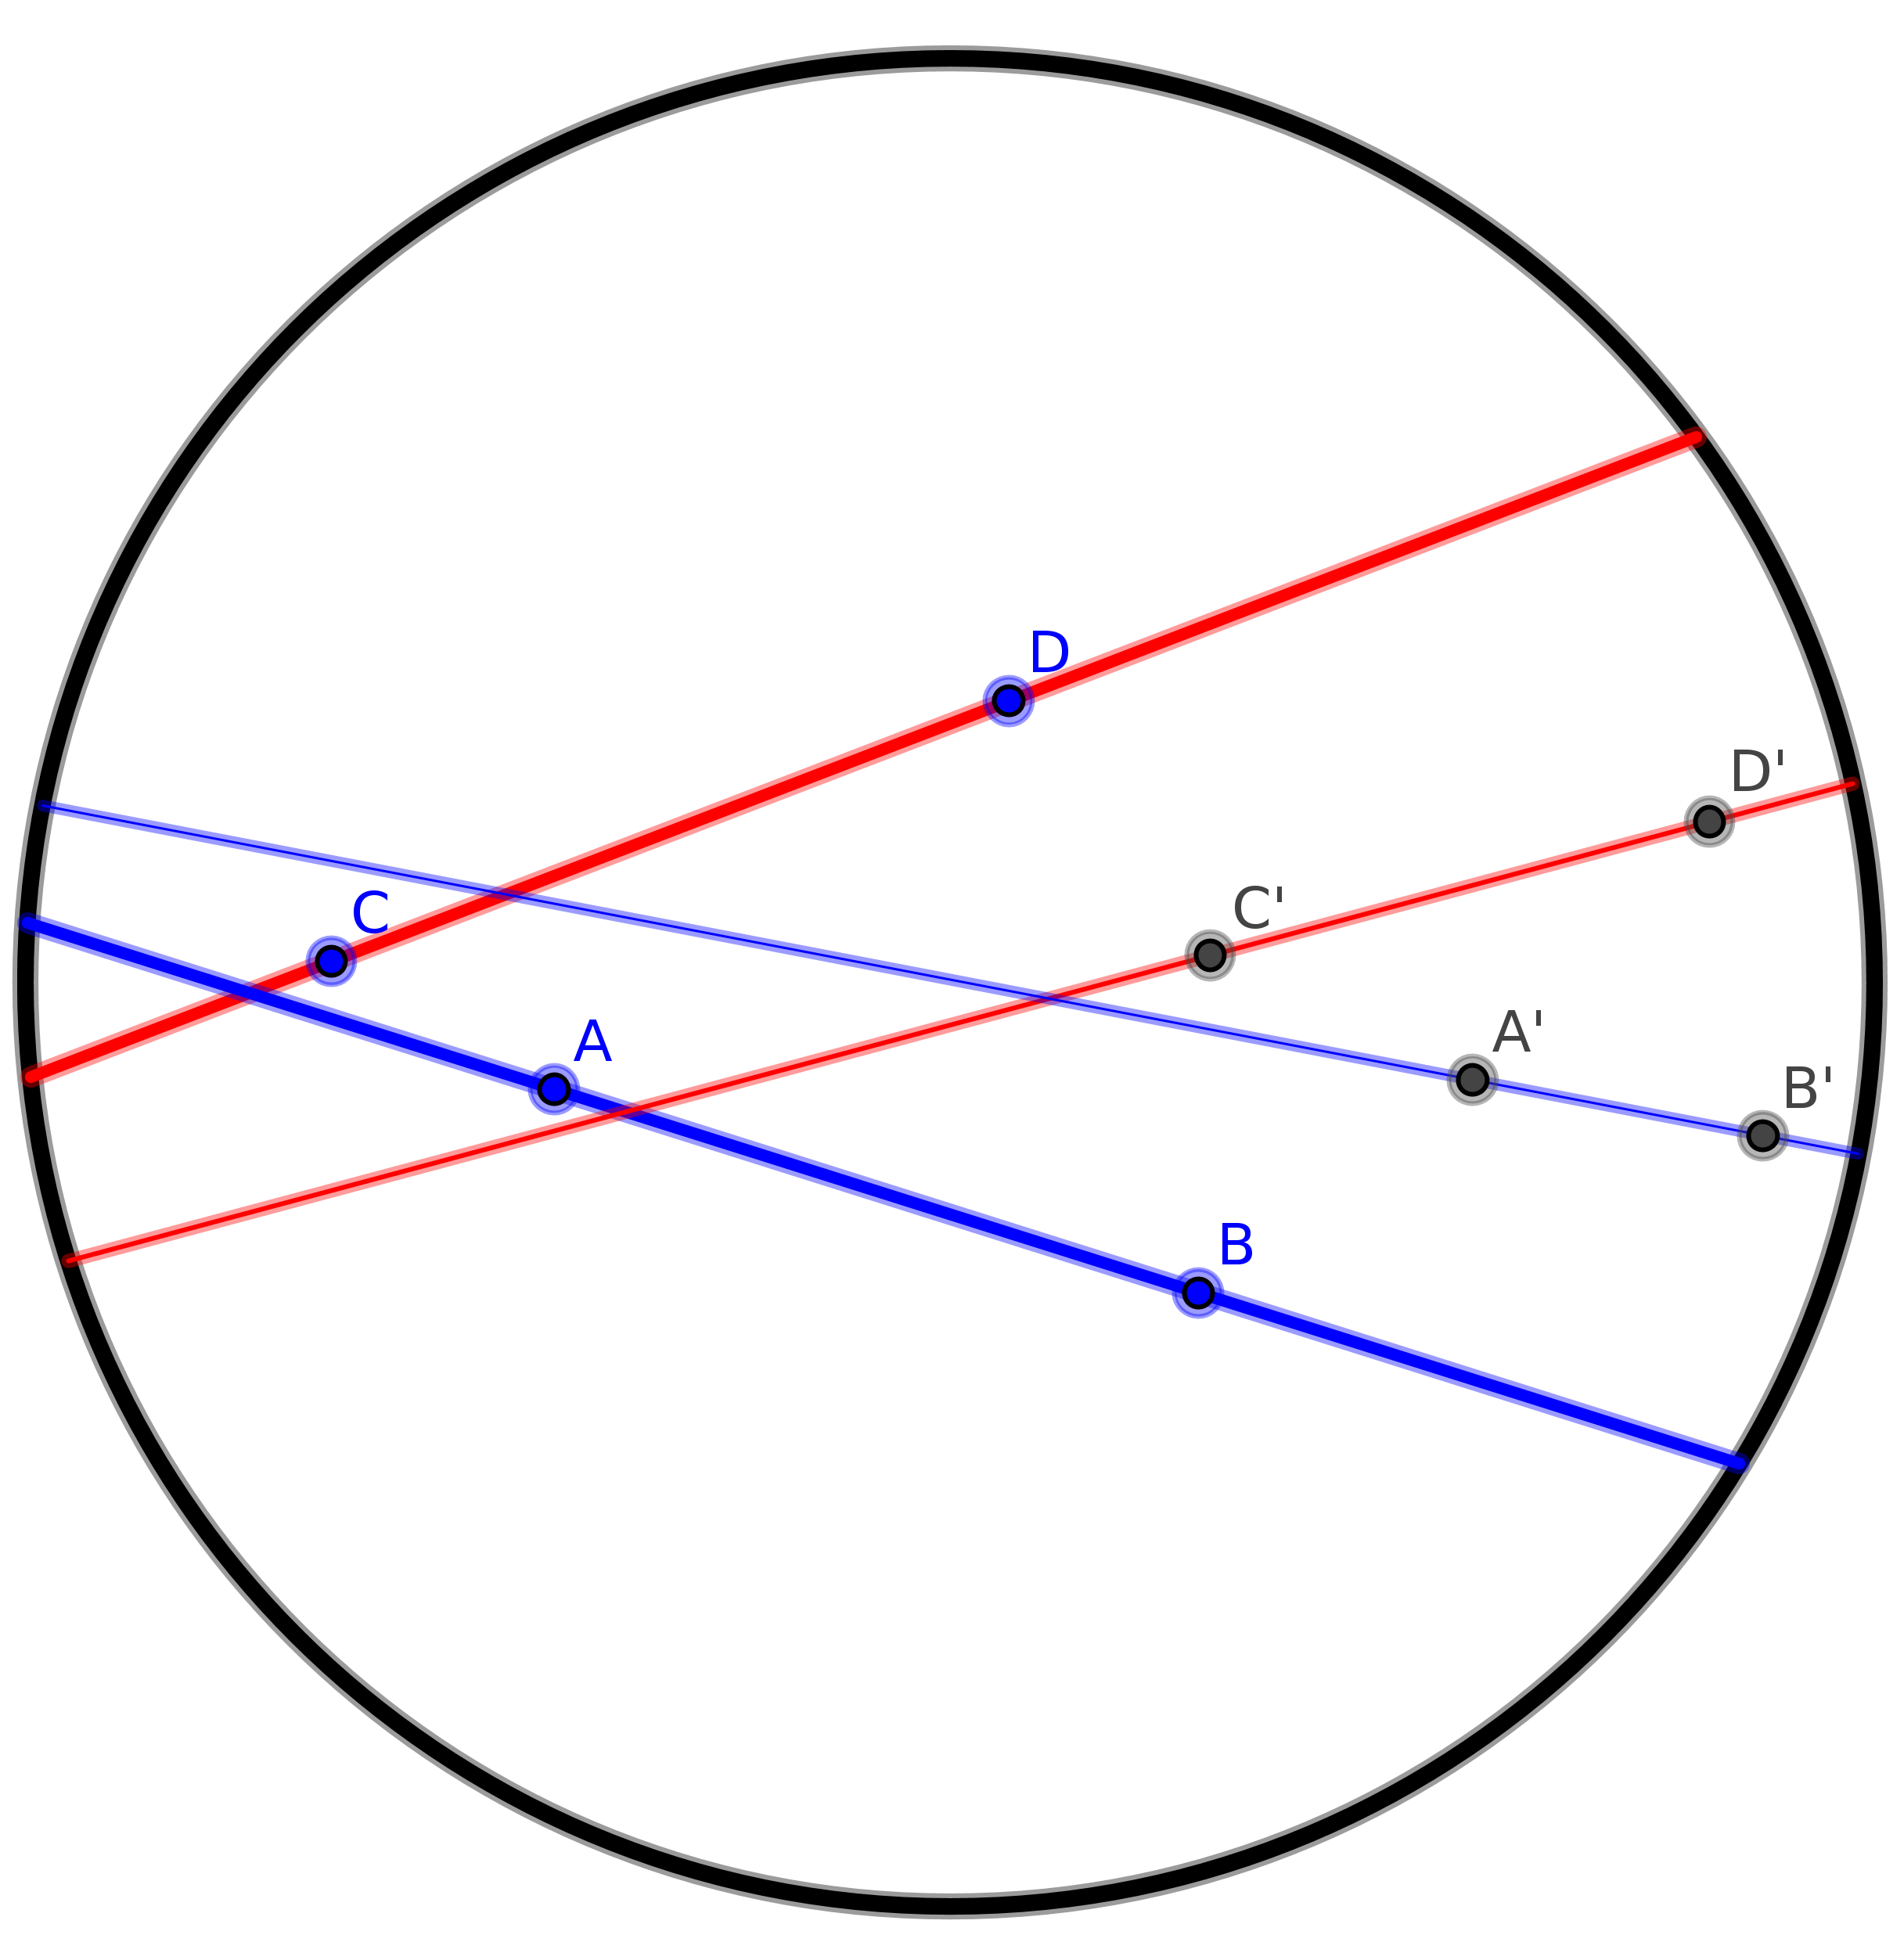
\includegraphics[width=2.5in]{kleinDiskNonConformal.png}
  \end{image}
  where $\overline{A'B'}$ and $\overline{C'D'}$ are the images of
  $\overline{AB}$ and $\overline{CD}$ under a $K$-rigid
  motion. Explain how this image shows that central projection does
  not preserve angles.
\end{problem}


\section{Areas in central projection coordinates}



We have already seen that on the $R$-sphere, the area of an
$\alpha$-lune is $2\alpha\cdot R^2$. Let's compute this a different
way.

\begin{problem}
  Let $K>0$ and consider the following region in central projection
 \begin{image}
   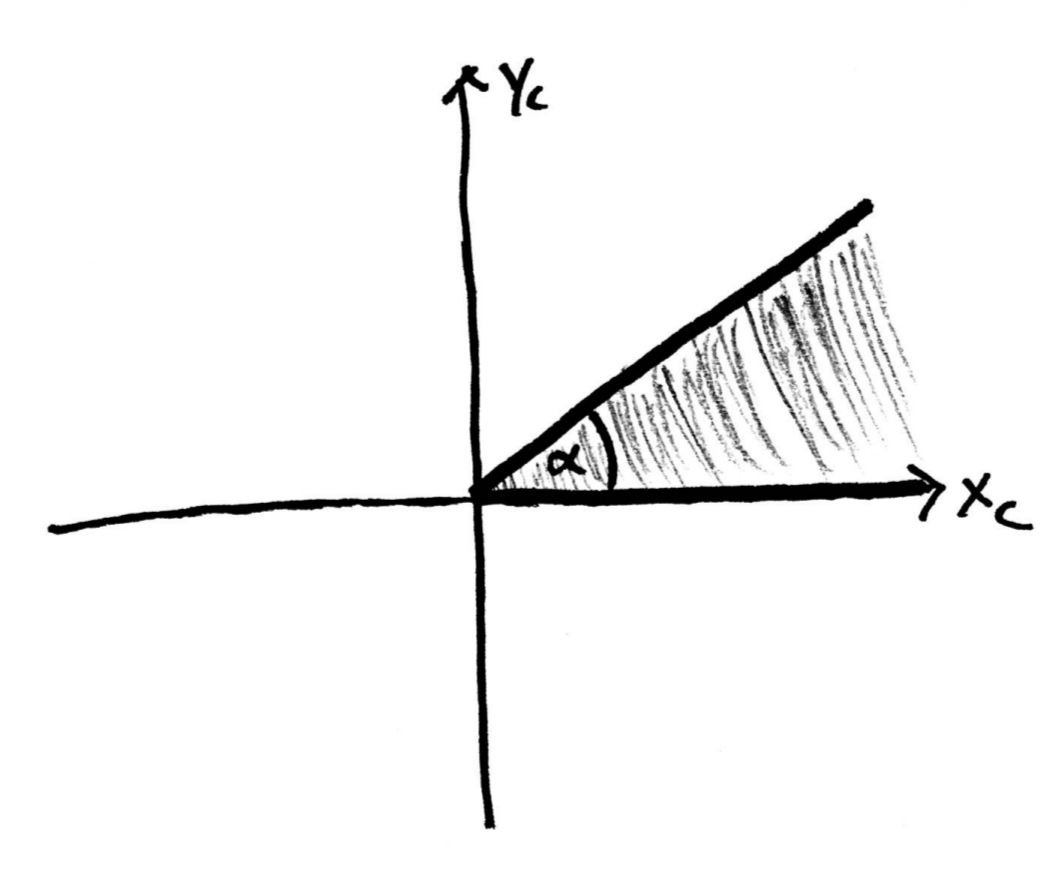
\includegraphics[width=3in]{halfLune.png}
 \end{image}
 Use the fact that the area of an $\alpha$-lune is $2\alpha\cdot R^2$
 to compute the area of the region.
\end{problem}

On the other hand, we know that the area in spherical geometry
represented by the region in central projection is given by
\[
\int_{L_c} \sqrt{
  \det
  \begin{bmatrix}
    \dd[X]{x_c}\bullet_K \dd[X]{x_c} & \dd[X]{y_c}\bullet_K \dd[X]{x_c} \\
    \dd[X]{x_c}\bullet_K \dd[X]{y_c} & \dd[X]{y_c}\bullet_K \dd[X]{y_c}
  \end{bmatrix}
}\d x_c\d y_c
\]

\begin{problem}
  Give a heuristic explanation of why this integral computes what we
  say it computes.
\end{problem}

You have already shown that
\[
\int_{L_c} \sqrt{
  \det
  \begin{bmatrix}
    \dd[X]{x_c}\bullet_K \dd[X]{x_c} & \dd[X]{y_c}\bullet_K \dd[X]{x_c} \\
    \dd[X]{x_c}\bullet_K \dd[X]{y_c} & \dd[X]{y_c}\bullet_K \dd[X]{y_c}
  \end{bmatrix}
}\d x_c\d y_c
\]
\[
=
\int_{L_c} \sqrt{
  \det\left(
  \begin{bmatrix}
    \dd[X]{x_c}\\
    \dd[X]{y_c}
  \end{bmatrix}
  \begin{bmatrix}
    1 & 0 & 0\\
    0 & 1 & 0\\
    0 & 0 & K^{-1}
  \end{bmatrix}
  \begin{bmatrix}
    \left(\dd[X]{x_c}\right)^\transpose & \left(\dd[X]{y_c}\right)^\transpose
  \end{bmatrix}\right)
}\d x_c\d y_c
\]

\begin{problem}
  Explain why
  \[
\begin{bmatrix}
    \dd[X]{x_c}\\
    \dd[X]{y_c}
  \end{bmatrix}
  \begin{bmatrix}
    1 & 0 & 0\\
    0 & 1 & 0\\
    0 & 0 & K^{-1}
  \end{bmatrix}
  \begin{bmatrix}
    \left(\dd[X]{x_c}\right)^\transpose & \left(\dd[X]{y_c}\right)^\transpose
  \end{bmatrix} =P_c.
  \]
  \begin{hint}
    No new computations need to be done, just look at how $P_c$ was derived.
  \end{hint}
\end{problem}

Hence now we see 
\[
\int_{L_c} \sqrt{
  \det
  \begin{bmatrix}
    \dd[X]{x_c}\bullet_K \dd[X]{x_c} & \dd[X]{y_c}\bullet_K \dd[X]{x_c} \\
    \dd[X]{x_c}\bullet_K \dd[X]{y_c} & \dd[X]{y_c}\bullet_K \dd[X]{y_c}
  \end{bmatrix}
}\d x_c\d y_c = \int_{L_c} \sqrt{\det P_c}\d x_c\d y_c
\]
\begin{problem}
  Compute $\sqrt{\det P_c}$.
  \begin{hint}
    As a gesture of friendship, we'll remind you that
    \[
 P_c =
     \begin{bmatrix}
       \left(Ky_c^2+1\right)\lambda^4 & -Kx_{c}y_{c}\lambda^4\\
       -Kx_{c}y_{c}\lambda^4 & \left(Kx_c^2+1\right)\lambda^4
     \end{bmatrix} = \lambda^4 \cdot \begin{bmatrix}
       Ky_c^2+1 & -Kx_{c}y_{c}\\
       -Kx_{c}y_{c} & \left(Kx_c^2+1\right)
     \end{bmatrix}.
    \]
  \end{hint}
  \begin{freeResponse}
    Write
    \begin{align*}
    \det P_c &= \lambda^4\cdot \det \begin{bmatrix}
       Ky_c^2+1 & -Kx_{c}y_{c}\\
       -Kx_{c}y_{c} & \left(Kx_c^2+1\right)
    \end{bmatrix}\\
    &= \lambda^4\cdot\left(\left( Ky_c^2+1\right)\left(Kx_c^2+1\right) - K^2x_{c}^2y_{c}^2\right)\\
    &= \lambda^4\cdot\left(K^2x_{c}^2y_{c}^2 + Ky_c^2+Kx_c^2+1-K^2x_{c}^2y_{c}^2\right)\\
    &= \lambda^4\cdot\left(Ky_c^2+Kx_c^2+1\right)
    \end{align*}
    However, $\lambda = \frac{1}{K\left(x_c^2+y_c^2\right)+1}$, so
    \[
    \sqrt{\det P_c} = \frac{1}{\left(K\left(x_c^2+y_c^2\right)+1\right)^{3/2}}.
    \]
  \end{freeResponse}
\end{problem}

At this point we see we are interested in the following integral
\[
\int_{L_c} \frac{1}{\left(K\left(x_c^2+y_c^2\right)+1\right)^{3/2}} \d x_c\d y_c.
\]

\begin{problem}
  Examining the following diagram
  \begin{image}
    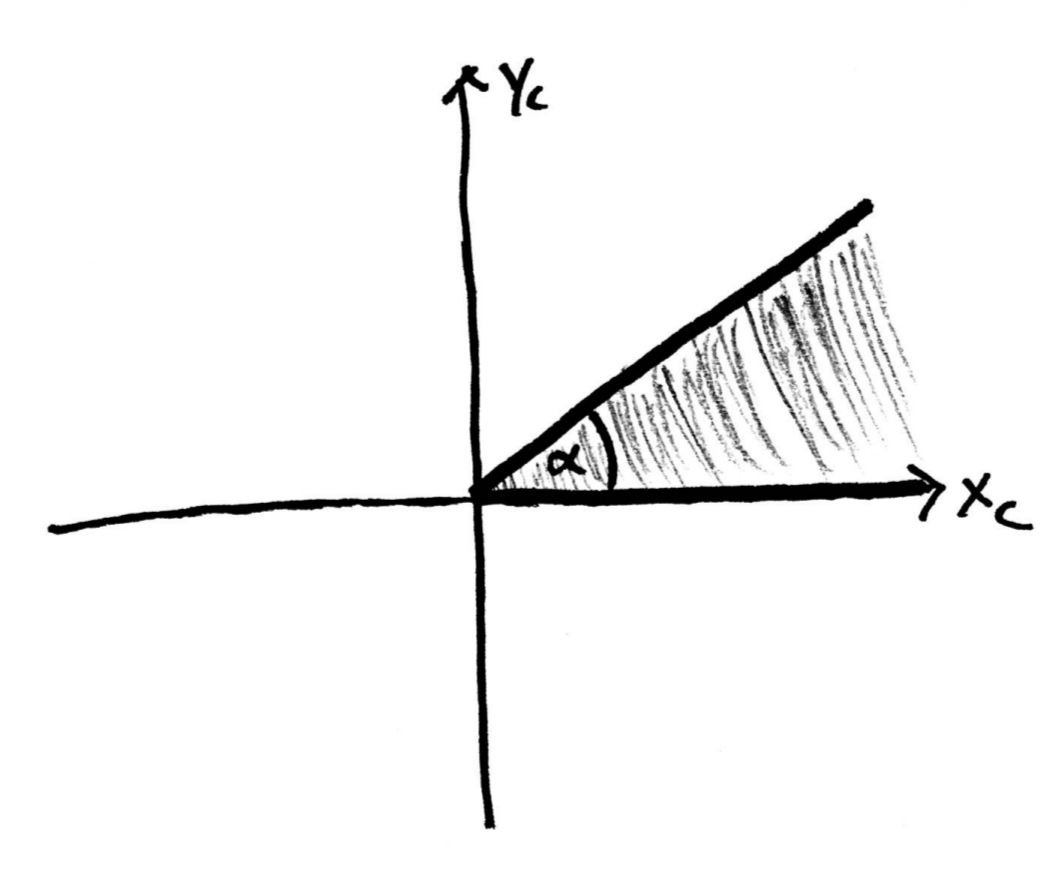
\includegraphics[width=3in]{halfLune.png}
  \end{image}
  convert
  \[
  \int_{L_c} \frac{1}{\left(K\left(x_c^2+y_c^2\right)+1\right)^{3/2}} \d x_c\d y_c.
  \]
  to polar coordinates and compute the integral.
  \begin{hint}
    Recall that to covert to polar coordinates, set
    \begin{align*}
      r &= \sqrt{x_c^2+y_c^2},\\
      \theta &= \arctan(y_c/x_c),
    \end{align*}
    and replace $\d x_c\d y_c$ with $r\d r\d \theta$.
  \end{hint}
  \begin{freeResponse}
    \[
    \int_{L_c}
    \frac{1}{\left(K\left(x_c^2+y_c^2\right)+1\right)^{3/2}} \d x_c\d
    y_c = \int_0^\alpha \int_0^\infty \frac{1}{\left(K\cdot r^2+1\right)^{3/2}} r\d r \d \theta.
    \]
    Integrating this from the inside-out we find
    \begin{align*}
      \int_0^\alpha \int_0^\infty \frac{1}{\left(K\cdot r^2+1\right)^{3/2}} r\d r \d \theta &= \int_0^\alpha \eval{\frac{-1}{K\left(K\cdot r^2+1\right)^{1/2}}}_0^\infty \d \theta\\
      &= \int_0^\alpha \frac{1}{K} \d \theta\\
      &= \frac{\alpha}{K}.   
    \end{align*}
    Recalling that $K = \frac{1}{R^2}$ we find our final answer is $\alpha \cdot R^2$.
  \end{freeResponse}
\end{problem}

\begin{problem}
  Reconcile this computation with what you know about the area of the
  $\alpha$-lune.
\end{problem}


\section{Central projection unifies euclidean, spherical, and hyperbolic geometry}

Under central projection, our new dot product defined by
\[
V_c\bullet_c W_c = V_c\cdot P_c\cdot W_c^\transpose
\]
make sense when $K$ is zero, positive, and negative. Hence this dot
product makes sense for euclidean, spherical, and hyperbolic
geometry. Moreover, in central projection, shortest paths on the $K$-surface
\[
K\left(x^2 + y^2\right) + z^2 = 1
\]
map to lines in the plane $z=1$. However, there is one trade-off:
Angles are not preserved in central projection. This means that when
angles are projected into the plane via central projection, the angle
we see in the $(x_c,y_c)$-plane may or may not be the actual angle
between two vectors. Summarizing, we have:



\[
{\renewcommand{\arraystretch}{2.7}
  \begin{tabular}{|c||c|c|c|}\hline
    & \begin{minipage}{2cm}\begin{center}Spherical ($K>0$)\end{center}\end{minipage} & \begin{minipage}{2cm}\begin{center}Euclidean ($K=0$)\end{center}\end{minipage} & \begin{minipage}{2cm}\begin{center}Hyperbolic ($K<0$)\end{center}\end{minipage}\\\hline\hline
    \begin{minipage}{2cm}\begin{center}Surface in \\ euclidean space\end{center}\end{minipage} & $\hat{x}^{2}+\hat{y}^{2}+\hat{z}^{2}=R^{2}$ & DNE  & DNE \\\hline
    \begin{minipage}{2cm}\begin{center}Euclidean dot product\end{center}\end{minipage} & $\hat{V}\cdot \hat{W}^\transpose$ & DNE  & DNE\\\hline
     \begin{minipage}{2cm}\begin{center}Surface in $K$-warped space\end{center}\end{minipage} & \multicolumn{3}{c|}{$1=K\left(  x^{2}+y^{2}\right)  +z^{2}$}\\\hline
     \begin{minipage}{2cm}\begin{center}$K$-dot product\end{center}\end{minipage} & $V\left[\begin{smallmatrix}1 & 0 & 0\\ 0 & 1 & 0\\ 0 & 0 & K^{-1}\end{smallmatrix}\right] W^\transpose$ &  DNE & $V\left[\begin{smallmatrix}1 & 0 & 0\\ 0 & 1 & 0\\ 0 & 0 & K^{-1}\end{smallmatrix}\right]W^\transpose$\\\hline
     \begin{minipage}{2cm}\begin{center}Central dot product\end{center}\end{minipage} & \multicolumn{3}{c|}{$V_c\cdot P_c\cdot W_c^\transpose = V_c\left[\begin{smallmatrix}\left(Ky_c^2+1\right)\lambda^4 & -Kx_{c}y_{c}\lambda^4\\
    -Kx_{c}y_{c}\lambda^4 & \left(Kx_c^2+1\right)\lambda^4\end{smallmatrix}\right] W_c^\transpose$}\\\hline
\end{tabular}}
\]




\begin{problem}
Summarize the results from this section. In particular, indicate which
results follow from the others.
\begin{freeResponse}
\end{freeResponse}
\end{problem}

\end{document}
